% !TeX root =../main.tex

\chapter{Concept and Implementation} \label{sec:cha3}
In this chapter, the realisation of three pre-built LTspice models to simulate non-ideal frequency behaviour, saturation and hysteresis is discussed, with the goal of creating a mix of these to best recreate the reality of the inductors behaviour. For each presented model first the method of inductor characterisation provided by LTspice is introduced. Then the tools and approaches used to extract the necessary parameters from the observed inductors are presented. Finally these parameters are inserted into LTspice and validated with the help of measurements from the corresponding buck converter. To avoid simulating an entire buck converter, the inductors are subjected to a periodic voltage, mirroring the behaviour of a synchronous buck converter. This removes the need to simulate the switching elements while keeping the excitation of the inductor the same. \\
The five inductors discussed in this chapter, listed in table \ref{tab:list_of_inductors}, are all products produced by Coilcraft and fall under the category of power inductors. These are designed to be used in SMPS and are therefore common in buck converters. 
\begin{table}[H]
    \centering
    \caption{List of Inductors}
    \begin{tabular}{|c|c|l|}
    \hline
    Inductor &  Inductance & Type \\
    \hline
     XGL1313-103ME & $10 \mu H$ & Molded Inductor \\
        XGL1313-223ME & $22 \mu H$ & Molded Inductor \\
        SER1512-103ME & $10 \mu H$ & High Current Flat Wire Inductor \\
        SER1512-223ME & $22 \mu H$ & High Current Flat Wire Inductor \\
        UA8014-AL & $2 \cdot 10 \mu H$ & Uncoupled Dual Inductors \\
    \hline
    \end{tabular}
    \label{tab:list_of_inductors}
\end{table}

\section{Frequency response of the inductor} \label{sec:frequency_response_of_the_inductor}
The first and simplest type of inserting non-idealities into the inductor Model of LTspice is with an \ac{ECM} simulating the frequency response of a real inductor. The base inductor already has an \ac{ECM} pictured in figure \ref{fig:inductor_ecm}. It takes into account the equivalent parallel capacitance between the individual windings of the inductor $EPC$, the copper resistance at low frequencies $ESR$ and the overall resistance during resonance $EPR$. It acts as a starting point to approximate the frequency response of an inductor and as later demonstrated, is enough to characterise the above-mentioned inductors frequency response fully.
\begin{figure}[H]
    \centering
    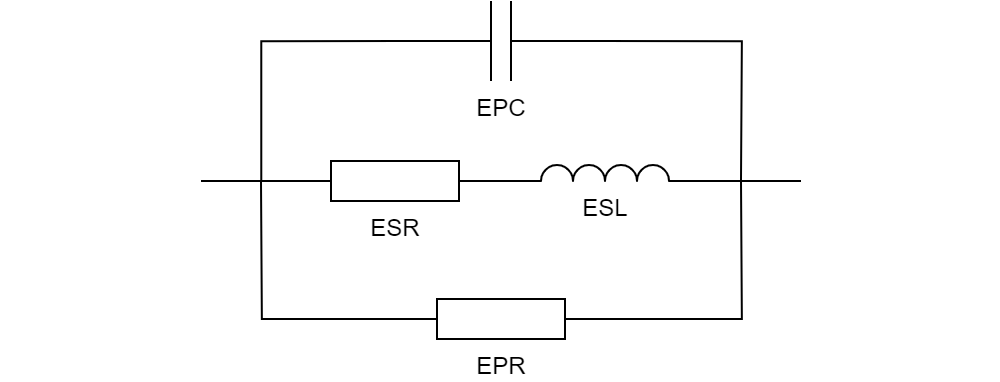
\includegraphics[width=0.70\linewidth]{Bilder//Kapitel3/Inductor_ECM.png}
    \caption{Inductor \ac{ECM}}
    \label{fig:inductor_ecm}
\end{figure}
To accurately measure the inductors frequency response a "Bode 100" by omicron-lab was used. It functions by subjecting the device under test to a sinusoidal frequency sweep from \SI{1}{\Hz} to \SI{50}{\Hz} and measuring its scattering parameters for every frequency. With this data gain, phase, inductance and quality factor are plotted in figgure \ref{fig:bode_100_measurements} and the values for the \ac{ECM} are calculated. Starting out close to purely resistive, the plot shows a shift to inductive behaviour at around \SI{10}{\kilo\Hz}, with magnitude increasing proportional to frequency and the phase approaching \SI{90}{\degree}. At the point of resonance, there is once again a short moment of pure resistive behaviour, after which the inductor begins to act like a capacitor, its magnitude decreasing and phase reaching negative \SI{90}{\degree}.\\
Applying this the inductance and series resistance can simply be read from the two graphs at the lowest available frequency. While for this inductor, the phase at this point still isn't zero and therefore inductive properties remain, the approximation still holds true, as both magnitude and phase level out before this point. Parallel capacitance and resistance are determined by the point of resonance. For this inductor, the resonant point lies at \SI{14,725}{\mega\Hz} with a pure resistance of \SI{5,582}{\kilo$\Omega$}. This resistance defines the parallel resistance of the \ac{ECM}. As resonance happens at the point, where the inductive reactance and capacitive reactance are equal, the capacitance can be determined by equation \ref{eq:ecm_capacitance}.
\begin{equation}\label{eq:ecm_capacitance}
    C_P = \frac{1}{\left(2 \pi \cdot f_r\right)^2\cdot L}
\end{equation}
\begin{figure}[H]
    \begin{subfigure}[b]{0.50\textwidth}
        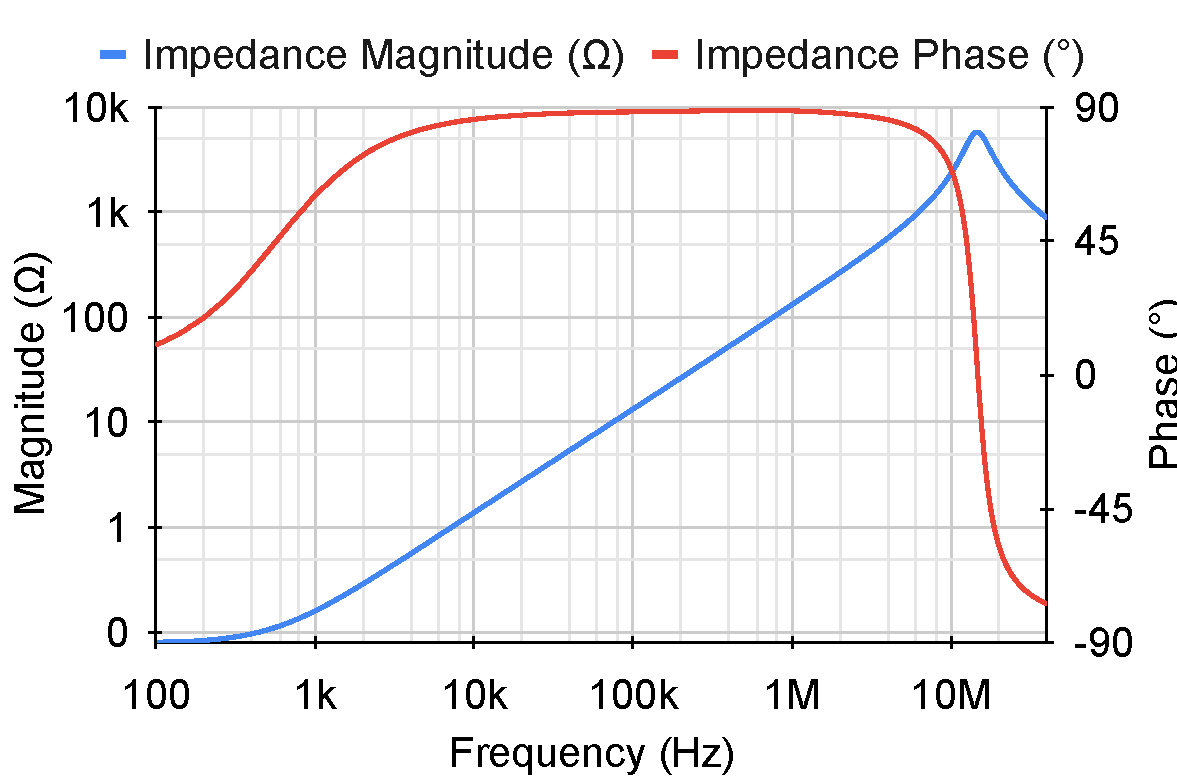
\includegraphics[width=\textwidth]{Bilder/Kapitel3/SER223_BodePlot.pdf}
        \caption{SER1512-223ME complex magnitude and phase vs frequency}
    \end{subfigure}
    \begin{subfigure}[b]{0.50\textwidth}
        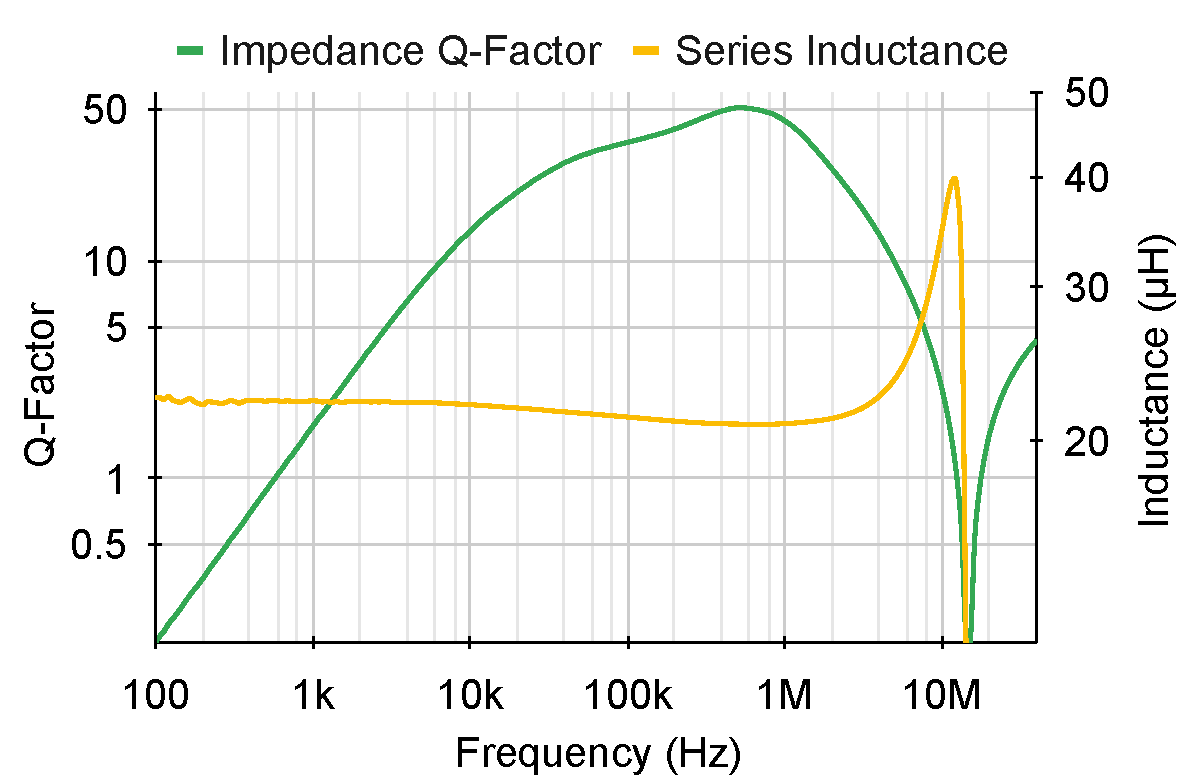
\includegraphics[width=\textwidth]{Bilder/Kapitel3/SER223_QLPlot.pdf}
        \caption{SER1512-223ME Q-factor and inductance vs frequency}
    \end{subfigure}
    \caption{Bode 100 measurement results for the SER1512-223ME}
    \label{fig:bode_100_measurements}							
\end{figure}
Comparing the results of the measurements and the LTspice simulation of figure \ref{fig:bode_100_measurements} and \ref{fig:LTspice_Frequency_Response}, the \ac{ECM} closely models the true frequency response, justifying its use. While impedance magnitude and phase match close to perfectly, the q-factor and inductance however stray from the true values. This can be attributed to the frequency dependence of the inductance, which is not separately modeled in the simulation. 
Using this approach, all five inductors were modelled and implemented in LTspice with similar results to the ones presented. In chapter \ref{sec:cha4} these models are validated via a buck converter.

\begin{figure}[H]
    \begin{subfigure}[b]{0.50\textwidth}
        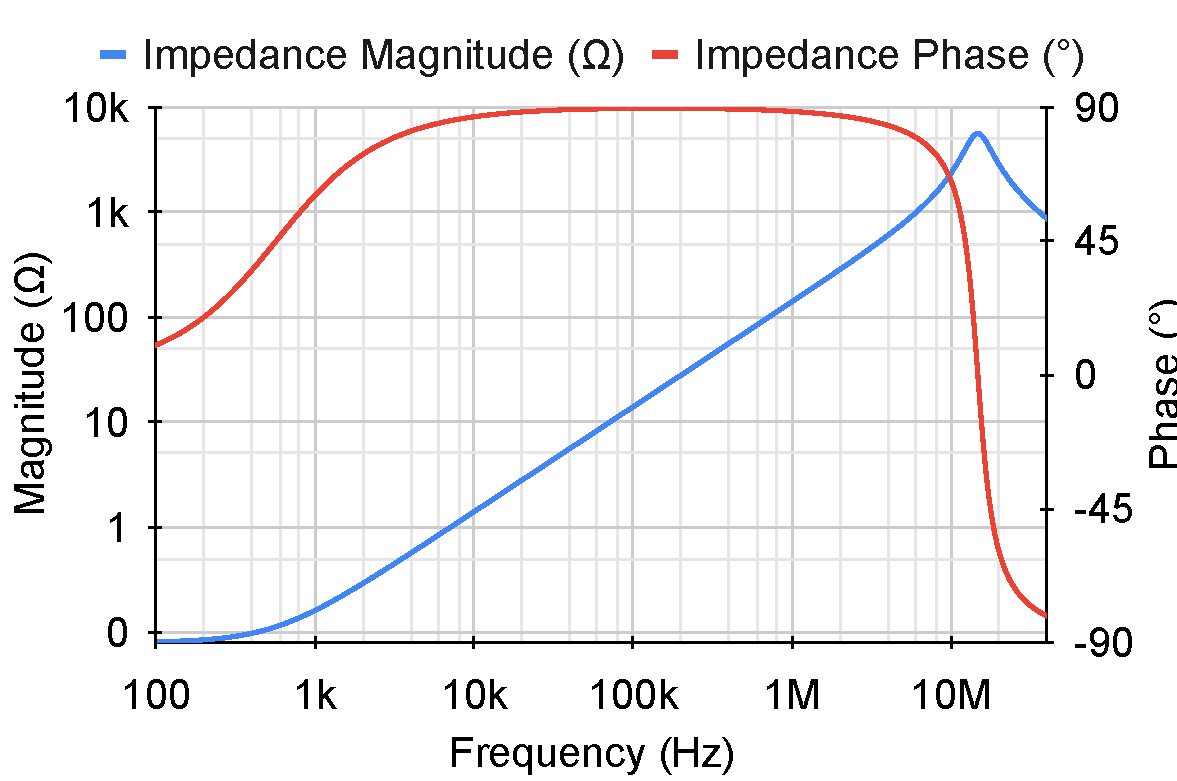
\includegraphics[width=\textwidth]{Bilder/Kapitel3/SER223_BodePlot_Spice.pdf}
        \caption{SER1512-223ME complex magnitude and phase vs frequency}
    \end{subfigure}
    \begin{subfigure}[b]{0.50\textwidth}
        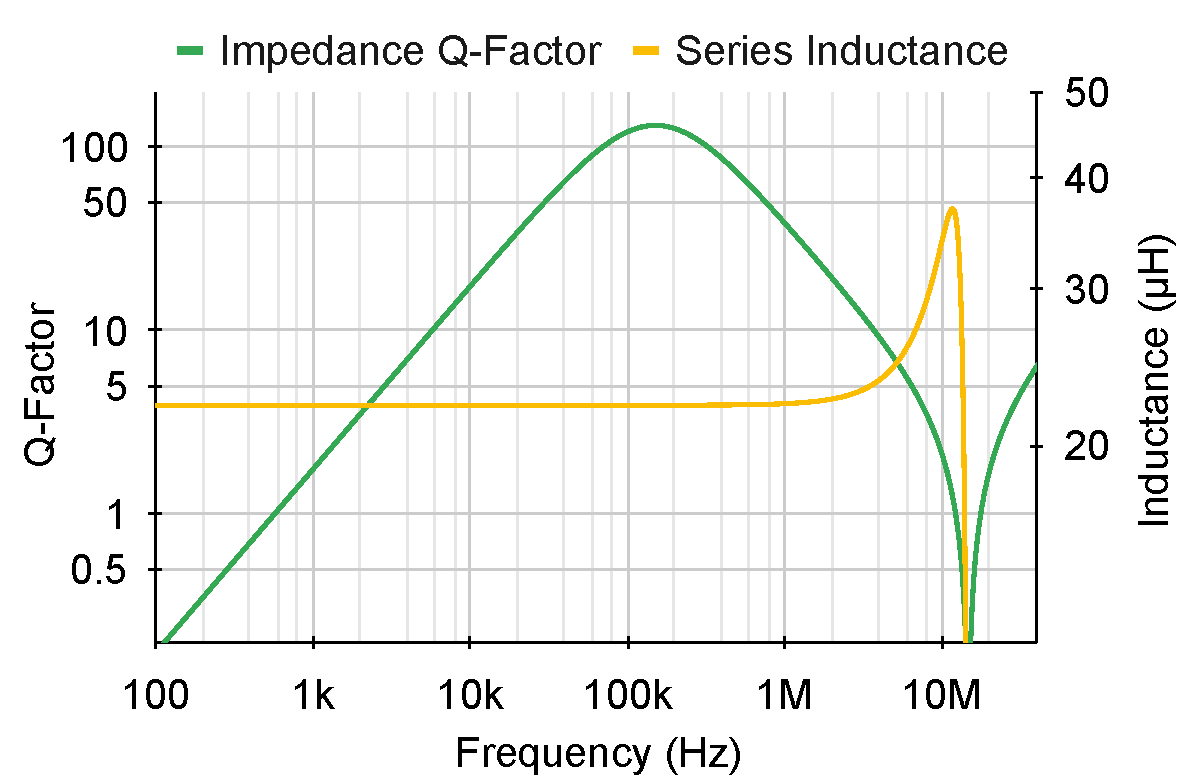
\includegraphics[width=\textwidth]{Bilder/Kapitel3/SER223_QLPlot_Spice.pdf}
        \caption{SER1512-223ME Q-factor and inductance vs frequency}
    \end{subfigure}
    \caption{Result of the LTspice simulation}
    \label{fig:LTspice_Frequency_Response}
\end{figure}

%Quelle:https://www.omicron-lab.com/products/vector-network-analysis/bode-100/technical-data

\section{Saturation behaviour of the inductor}\label{sec:saturation_behaviour_of_the_inductor}
The second type of inductor loss modelling takes advantage of the LTspice inbuilt \textit{flux} function. With it a  specific saturation curve can be input into the inductor, modelling the current dependence of the inductance. As this model does not influence the frequency behavior of the inductor, it is to be used in combination with the results from section \ref{sec:frequency_response_of_the_inductor}. \\
To measure the current dependant behaviour a "Power Choke Tester" by ed-k was used. It subjects the inductor under test to a rectangular voltage pulse and measures the current through it until a set current is reached. The voltage applied is set to be similar to the actual voltage the inductor is subjected to. With the voltage and current data, the device is able to calculate the magnetic flux in the inductor. Calculating the inductance is then done by differentiating the flux. The inductance of the SER1512-223ME inductor is displayed in figure \ref{fig:differential_inductance_of_the_ser1512-223me_inductor}. A close to constant inductance with an average of \SI{21.8}{\micro\henry} can be measured up to a current of \SI{5}{\A}, after which the curve decreases following an s-curve. Levelling out at an inductance around \SI{1.18}{\micro\henry}. This means that the inductor enters saturation at around \SI{5}{\A} of \ac{DC} through it, marking this current as the maximum current the inductor should experience without increasing the ripple current and causing greater power losses. 
\begin{figure}[H]
    \centering
    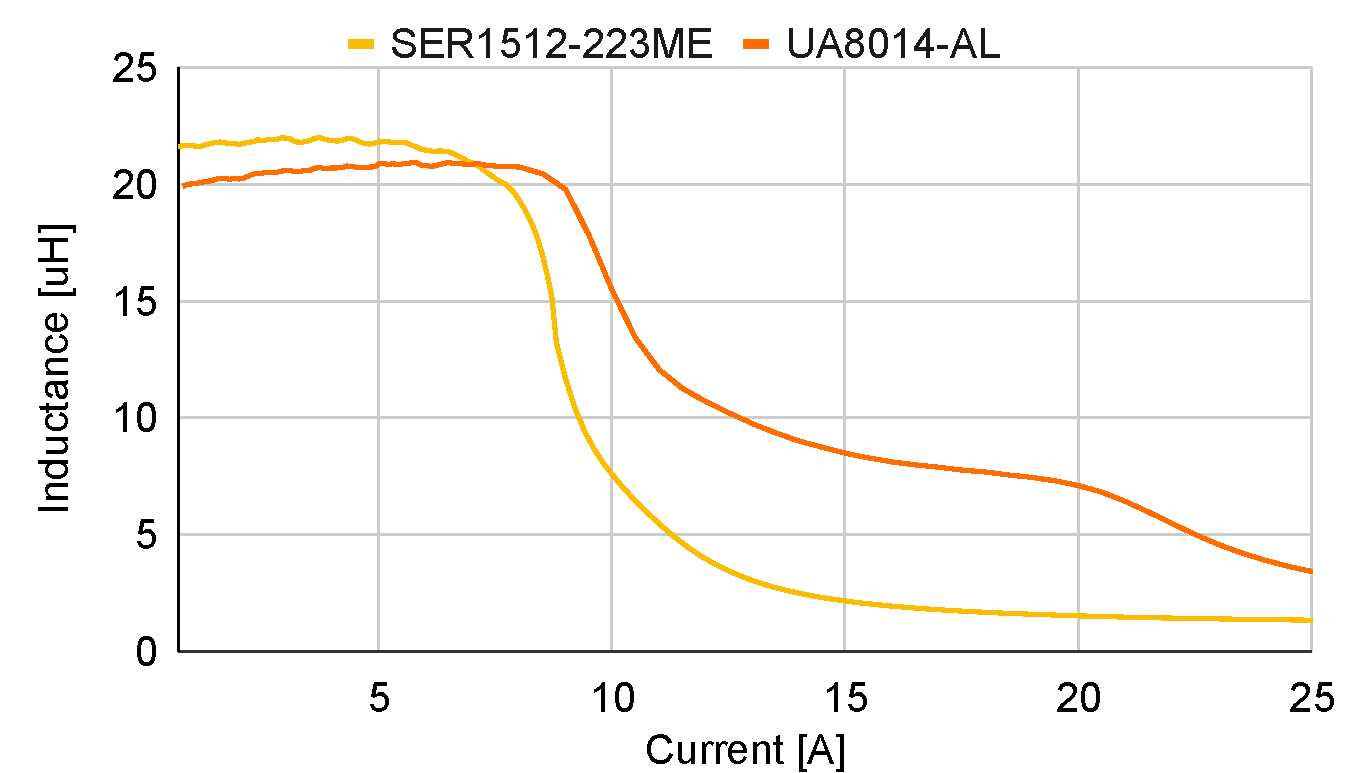
\includegraphics[width=0.75\linewidth]{Bilder//Kapitel3/SER223_UA_Saturation.pdf}
    \caption{Differential inductance of the SER1512-223ME and UA8014-AL inductor}
    \label{fig:differential_inductance_of_the_ser1512-223me_inductor}
\end{figure}
Crucial for the simulated inductor is the current behaviour of the inductance. Importing the measured flux value by value directly into LTspice is no option, as both the number of values is limited and the runtime of the simulation is drastically increased. Furthermore interpolating the measured flux and importing the result as a function is prone to errors, as already small deviations cause a noticeable difference in the inductance. Instead, curves are fitted to best describe the inductance for each inductor. A combination of different degree polynomials and exponential functions define a partwise function that approximates the saturation behaviour of the inductance. Integrating this function yields the flux curve, which can then be imported into LTspice using the \textit{flux}-command of the inductor.\\
Measuring the inductance curve of the inductor is done by subjecting it to an \ac{AC} with an amplitude of $\frac{1}{2\pi}$\SI{ }{\A}, frequency of \SI{1}{\Hz} and a varying \ac{DC} offset. The chosen amplitude and frequency enable the inductance to be determined by measuring the voltage across the inductor. As the inductors voltage is the product of the \ac{AC} amplitude and the inductors complex impedance, the frequency factor of $2\pi$ and the currents amplitude, cancel out as shown in equation \ref{eq:inductance_from_voltage}, resulting in the voltage being numerically equivalent to the inductance.
\begin{equation}\label{eq:inductance_from_voltage}
    \hat{V_L} = \hat{I_L} \cdot j 2\pi f\cdot L \triangleq L
\end{equation}

Comparing the inductance curve of the UA8014-AL inductor when measured and simulated, the flexibilty and precission of this approach can be well demonstrated. The fitted curve consisting of many partwise defined functions is able to closely follow the measured inductance. It is able to sensibly extend the inductance curve up to \SI{0}{\A} of current and also removes high frequency measurement noise visible in the low amperage range of the measured inductancec curve. Furthermore it has the advantage of causing no noticeable increase to the simulation runtime when compared to a model not taking advante of the \textit{flux}-command. 
\begin{figure}[H]
    \centering
    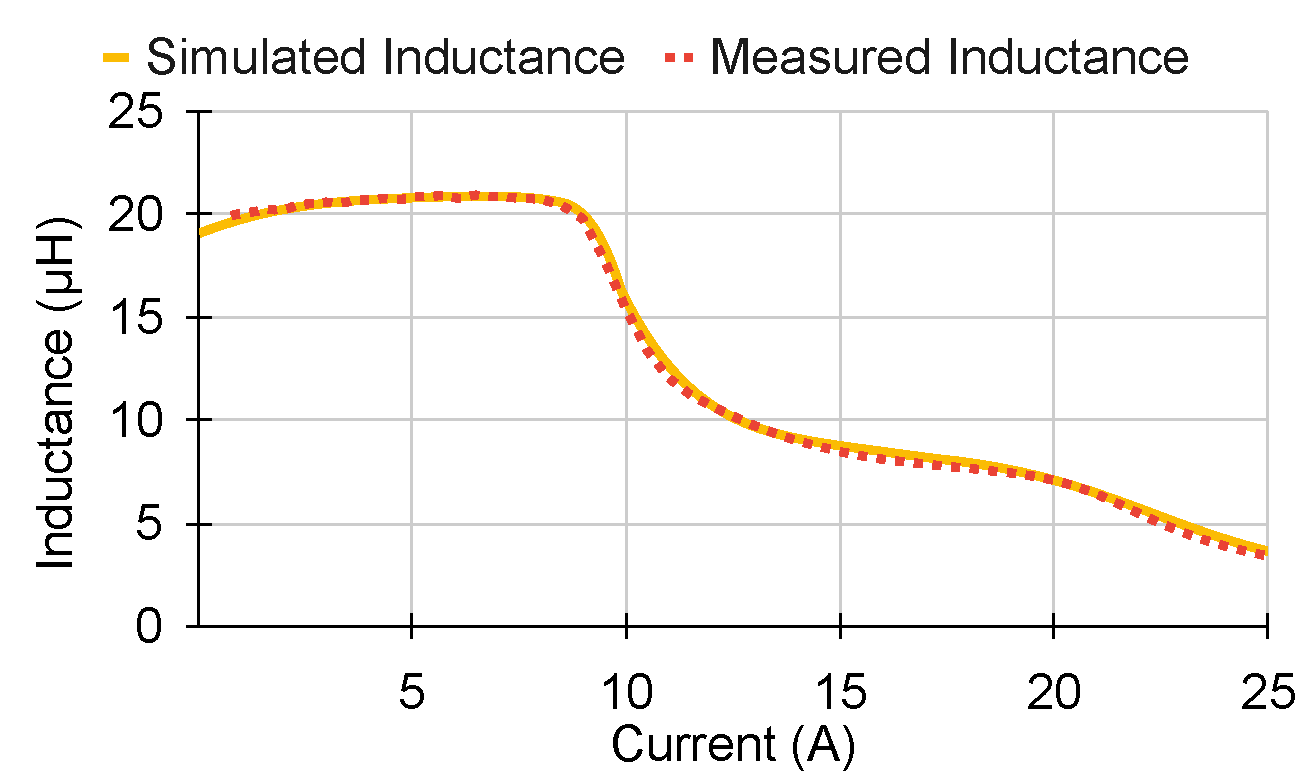
\includegraphics[width=0.6\linewidth]{Bilder/Kapitel3/Saturation_Measured_vs_LTspice.pdf}
    \caption{Comparison of the Inductance curve of the UA8014-AL measured and simulated}
    \label{fig:comparison_of_saturation}
\end{figure}

\newpage
\section{Hysteresis behavior of the inductor} \label{sec:hysteresis_behaviour_of_the_inductor}
The third type of inductor modelling provided by LTspice is hysteresis modelling. In contrast to the saturation model, it takes the \ac{DC} offset into account with the hope of modeling the inductor behaviour at high output currents accurately.\\
In contrast to the flux, where a function can be directly input in LTspice, the hysteresis curve is defined via seven parameters: Number of turns, length of the magnetic core, length of the air gap, crossectional area of the core, maximum B-field, remnant B-field and coercivity. The last three of these directly define the shape of the hysteresis curve, while the others are needed to calculate the inductance based on the hysteresis. Measuring the hysteresis is done using the same principle, the power choke tester of section \ref{sec:saturation_behaviour_of_the_inductor} uses, subjecting the inductor to a rectangular voltage pulse until the core reaches saturation. after which, the current is able to drop again. Since however there was no dedicated device available, this setup, displayed in figure \ref{fig:hysteresis_measurement_setup}, needed to be implemented manually.\\
\begin{figure}[H]
    \centering
    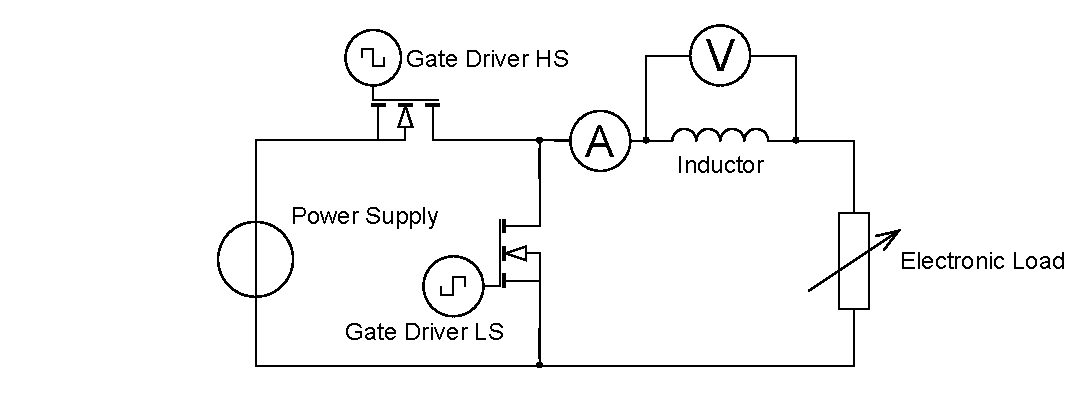
\includegraphics[width=.8\linewidth]{Bilder/Kapitel3/Hysteresis_Measurement_Setup.pdf}
    \caption{Hysteresis measurement setup}
    \label{fig:hysteresis_measurement_setup}
\end{figure}
Connecting the inductor under test to a \ac{GaNFET} half-bridge and adding a load with capacitive and resistive properties, allows the charging time to be regulated and a reverse current to flow through the inductor. The reverse current is necessary to measure the coercive force. Connecting a current clamp to the inductors connecting wire and a voltage probe across the inductor enables the oscilloscope to measure the B-H curve. The main limiting factor of this setup is the minimum speed the \ac{GaNFET} half-bridge can switch at. Being designed for high switching speeds, up from \SI{100}{\kilo\Hz}, comes with the downside of not being able to properly switch at \SI{10}{\kilo\Hz}, as the capacitor holding the charge to enable the gate to switch will discharge too quickly. As the voltage determines the rate of change of the inductor current, a lower switching frequency is desirable, as it allows a lower voltage to be used to achieve the same maximum current. 10kHz being the lowest frequency selectable, a higher voltage is necessary to reach a maximum current above the saturation current. The selected power source however not only has to supply this voltage but also be able to handle rapid changes in the supplied current. This limits the power sources available. Concerning the connected load, it has to be able to handle the great power spikes created. Furthermore the resistive load has to be small enough to allow the desired current to flow, as the maximum voltage is set by the power source.\\

The here used Tektronix Series 6 oscilloscope comes with a prebuilt function to directly measure a B-H curve. Achieving the proper scale of the B-H curve requires adding the number of turns, crossectional area and magnetic length into the settings of the oscilloscope. These values create a source for errors, as the inductors listed in table \ref{tab:list_of_inductors} come with little to no information about their core and windings. 
To provide a proof of concept and ensure that measurement errors in the dimensions of the inductor are not a factor, a custom inductor with known dimensions was used. A power inductor core from the producer ferroxcube, called PQ20/16, was chosen. Its measurements and core material are clearly defined and its core material datasheet also comes with the hysteresis curve, giving a point of comparison for the manual measurements. The core is wound with 8 windings and pressed together to create an inductor without an air gap. Hereby all variables for the hysteresis measurement are known and listed in the table \ref{tab:parameters_of_the_custom_inductor}. \\
\begin{table}[H]
    \centering
    \caption{Parameters of the custom inductor}
    \begin{tabular}{|l|c|c|c|c|}
        \hline
        Parameter & Magnetic length $l_m$ &  Air gap length $l_g$ &  Effective area $A_e$ & Windings $N$ \\
        \hline
        Value & \SI{37.8}{\milli\m} & \SI{0}{\milli\m} & \SI{61.9}{\milli\square\m} & 8\\
        \hline
    \end{tabular}
    \label{tab:parameters_of_the_custom_inductor}
\end{table}
Inserting this inductor into the measurement setup shown in figure \ref{fig:hysteresis_measurement_setup}, applying a \SI{52}{\V} supply voltage, allowing a maximum \SI{30}{\A} current pull and switching at \SI{13}{\kilo\Hz}, the behaviour shown in image \ref{fig:hysteresis_measurement_of_the_custom_wound_inductor} was created. 
Hysteresis and saturation behaviour are clearly visible. However, the noise at the points where the axes are crossed is substantial, influencing the values of the remnant B-field and the coercivity. Most of this noise is most likely measurement noise, as the oscilloscope needs to measure high voltages and currents, worsening the resolution at low currents and voltages. The distortion visible at the maximum point of saturation is due to fluctuations in the voltage of the power supply, as it operates at its peak capabilities.
\begin{figure}[H]
    \centering
    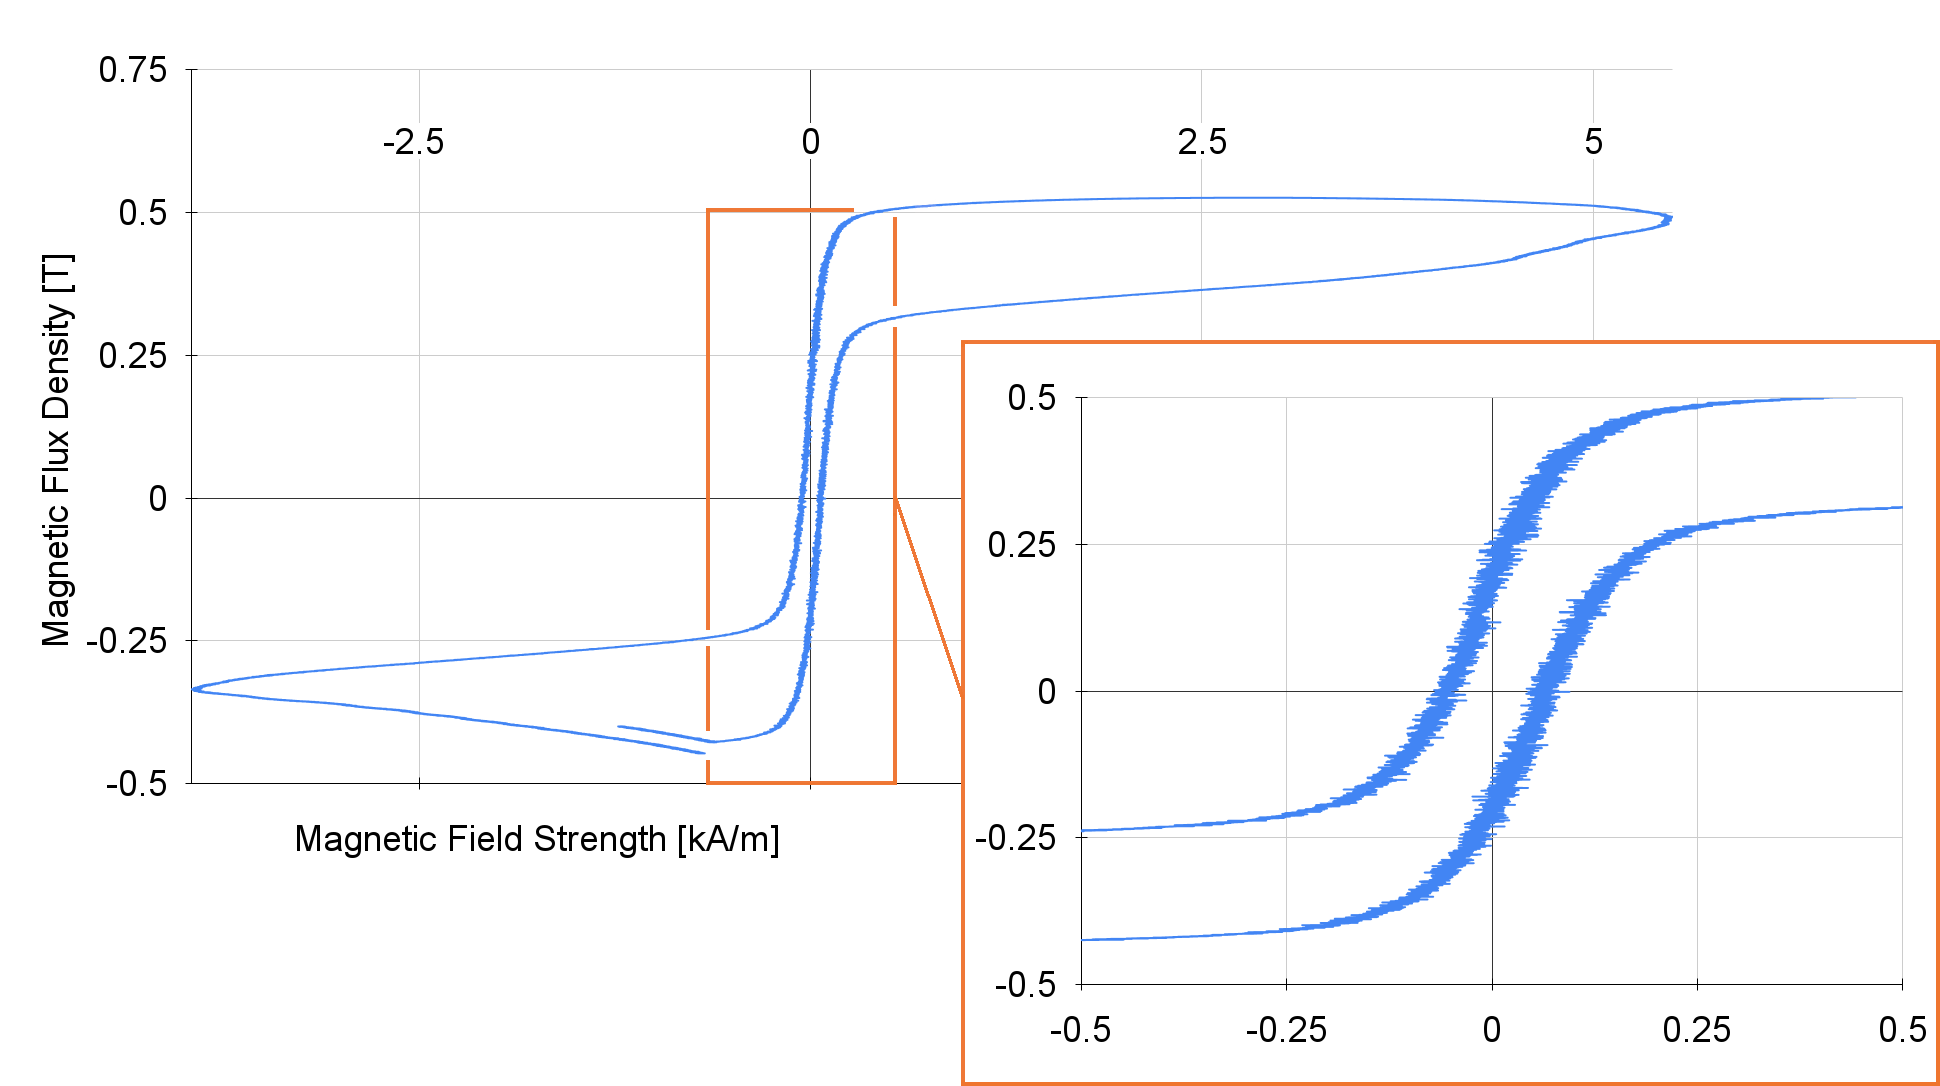
\includegraphics[width=1\linewidth]{Bilder//Kapitel3/Hysteresis_Measurement_3.png}
    \caption{Hysteresis Measurement of the custom wound inductor}
    \label{fig:hysteresis_measurement_of_the_custom_wound_inductor}
\end{figure}
Table \ref{tab:B-H_curve_points_of_interest_comparison} compares the measured points of interest to the data provided by the producer of the core material. While the deviations are significant, they are still attributable to the noise and limitations of the setup. If the setup is changed to allow for higher precision at low currents and voltages and the saturation region is not plagued by unwanted behaviour of the power supply and electronic load, the results can improve. Knowing that the B-H curve is measurable and its results, after appropriate changes to the setup, should match reality, the implementation in LTspice is now discussed.
\begin{table}[H]
    \centering
    \caption{B-H curve points of interest comparison}
    \begin{tabular}{|l|c|c|}
        \hline
        & Measured & Given by the datasheet \\
        \hline
        Coercive Force $H_c$ & \SI{54}{\A\per\m} & \SI{13}{\A\per\m}\\ 
        \hline
        Remnant B-Field $B_r$ & \SI{255}{\milli\tesla} & \SI{156}{\milli\tesla}\\
        \hline
        Maximum B-Field $B_{max}$ & \SI{570}{\milli\tesla} & \SI{500}{\milli\tesla}\\
        \hline
    \end{tabular}
    \label{tab:B-H_curve_points_of_interest_comparison}
\end{table}
To ensure that the use of ideal values in the LTspice simulation results in the desired behaviour and provides a proof of concept, the B-H curve is simulated purely with the values given by the cores datasheet, listed in table \ref{tab:parameters_of_the_custom_inductor} and table \ref{tab:B-H_curve_points_of_interest_comparison}. Verifying the LTspice simulation is done by plotting the B-H curve of the simulated inductor. For this a sinusoidal current is applied to the inductor with no \ac{DC} offset and at the same frequency as the datasheet uses, \SI{10}{\kilo\Hz}. The B- and H-field values are calculated through Faradays and Amperes law. Faradays law states, that a changing magnetic flux $\Phi$ induces a voltage in a wire loop with the cross-sectional area $A$. As the magnetic flux can be expressed as the product of the area $A$ and the magnetic flux density $B$ and the voltage is proportional to the number of loops of wire $N$, the equation can be rearranged to the expression \ref{eq:faradays_law} describing the B-field. 
\begin{equation}
	B = \frac{1}{N \cdot A} \int_0^t u(\tau)d\tau \label{eq:faradays_law}    
\end{equation}
In contrast, Amperes law describes that the magnetic field $H$ integrated along a closed loop is equal to the current enclosed by this loop. As in the core of an inductor, the magnetic field can be assumed to be constant and the length of the loop is given by the magnetic length $l_m$ of the core, the integral can be resolved. As the core encloses $N$ windings of the coil, the current creating the magnetic field is equal to the inflowing current $I$ times the number of windings. Solving for the magnetic field, results in equation \ref{eq:amperes_law}.
\begin{equation}
	H = I \cdot \frac{N}{l_m} \label{eq:amperes_law}
\end{equation}
Using behavioural voltage and current sources, the equations \ref{eq:faradays_law} and \ref{eq:amperes_law} can be directly implemented in LTspice, as they allow for functions and integration. The complete setup is seen in figure \ref{fig:hysteresis_measurement_setup_in_LTspice}. Plotting the voltage of the behavioural voltage source versus the current of the behavioural current source yields the simulated B-H curve shown in figure \ref{fig:hysteresis_comparison}.
\begin{figure}[H]
    \centering
    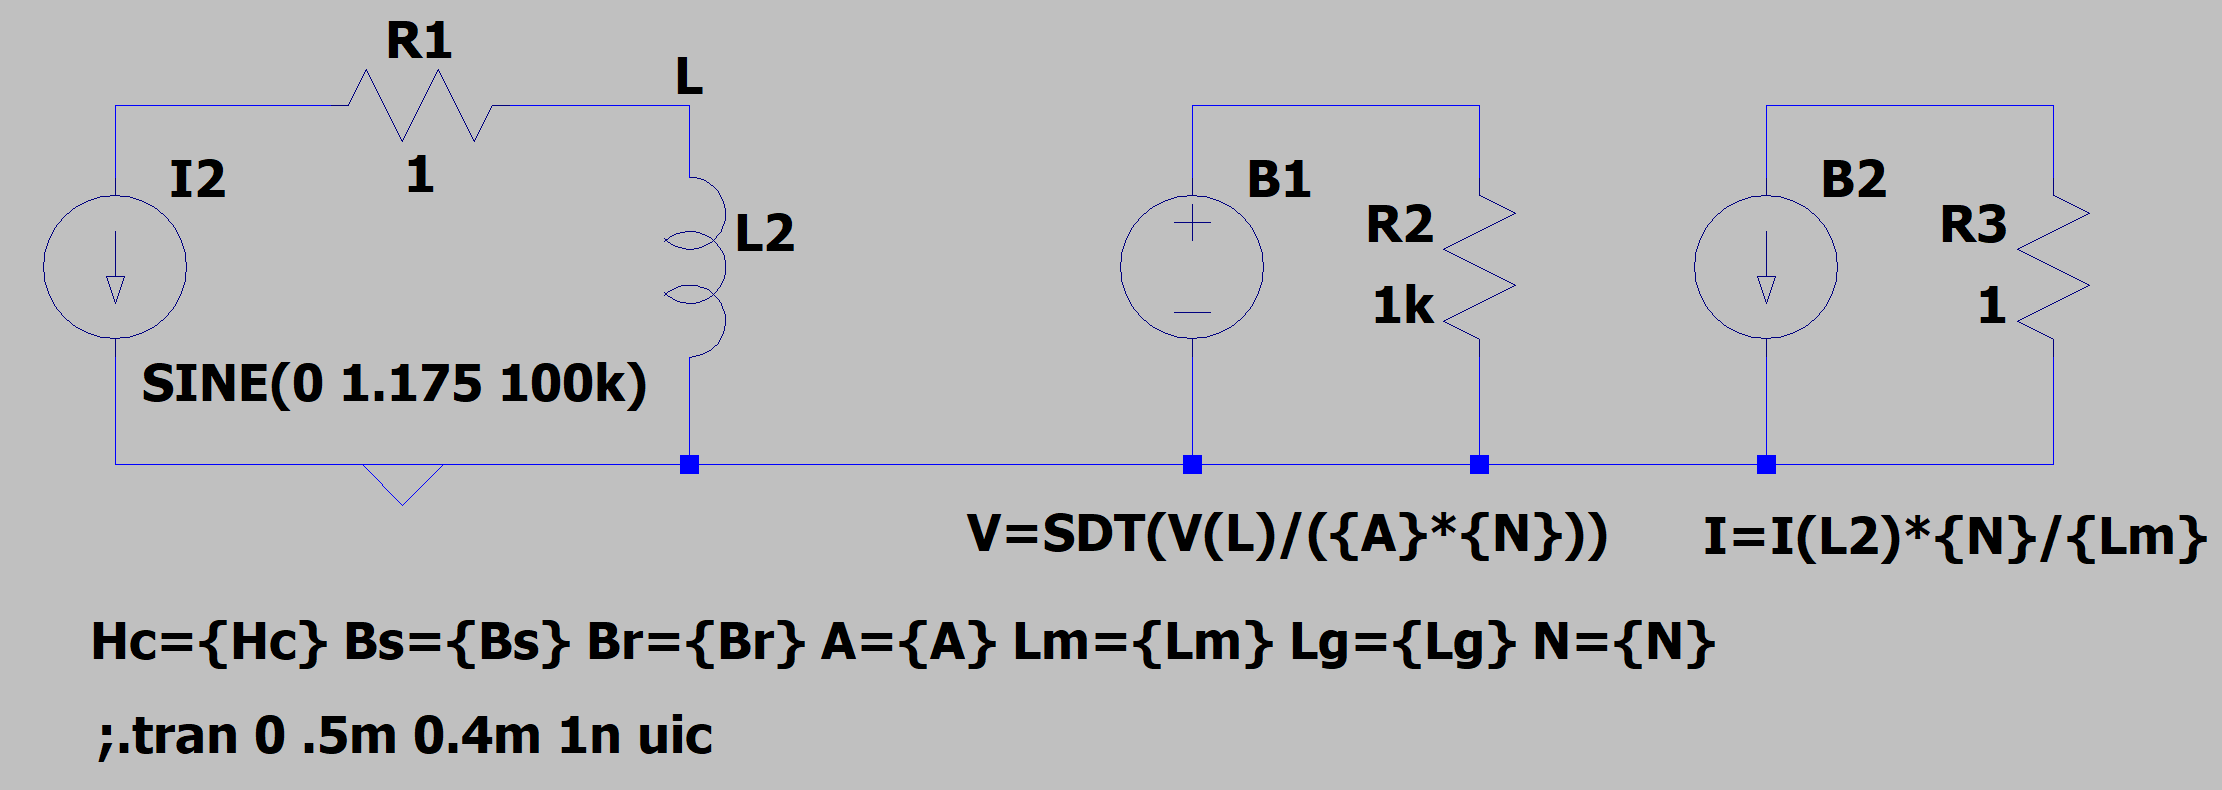
\includegraphics[width=.9\linewidth]{Bilder//Kapitel3/Hysteresis_Measurement_Setup_LTspice.png}
    \caption{Hysteresis measurement setup in LTspice}
    \label{fig:hysteresis_measurement_setup_in_LTspice}
\end{figure}
Mismatches are visible when comparing the simulated and provided B-H curves. While the simulated remnant B-field and coercivity only differ minimally from the input values, \SI{3}{\micro\tesla} and \SI{0.13}{\A\per\m} respectively, the maximum B-field differs substantially by \SI{50}{\milli\tesla}.
\begin{figure}[H]
    \begin{subfigure}[b]{0.50\textwidth}
        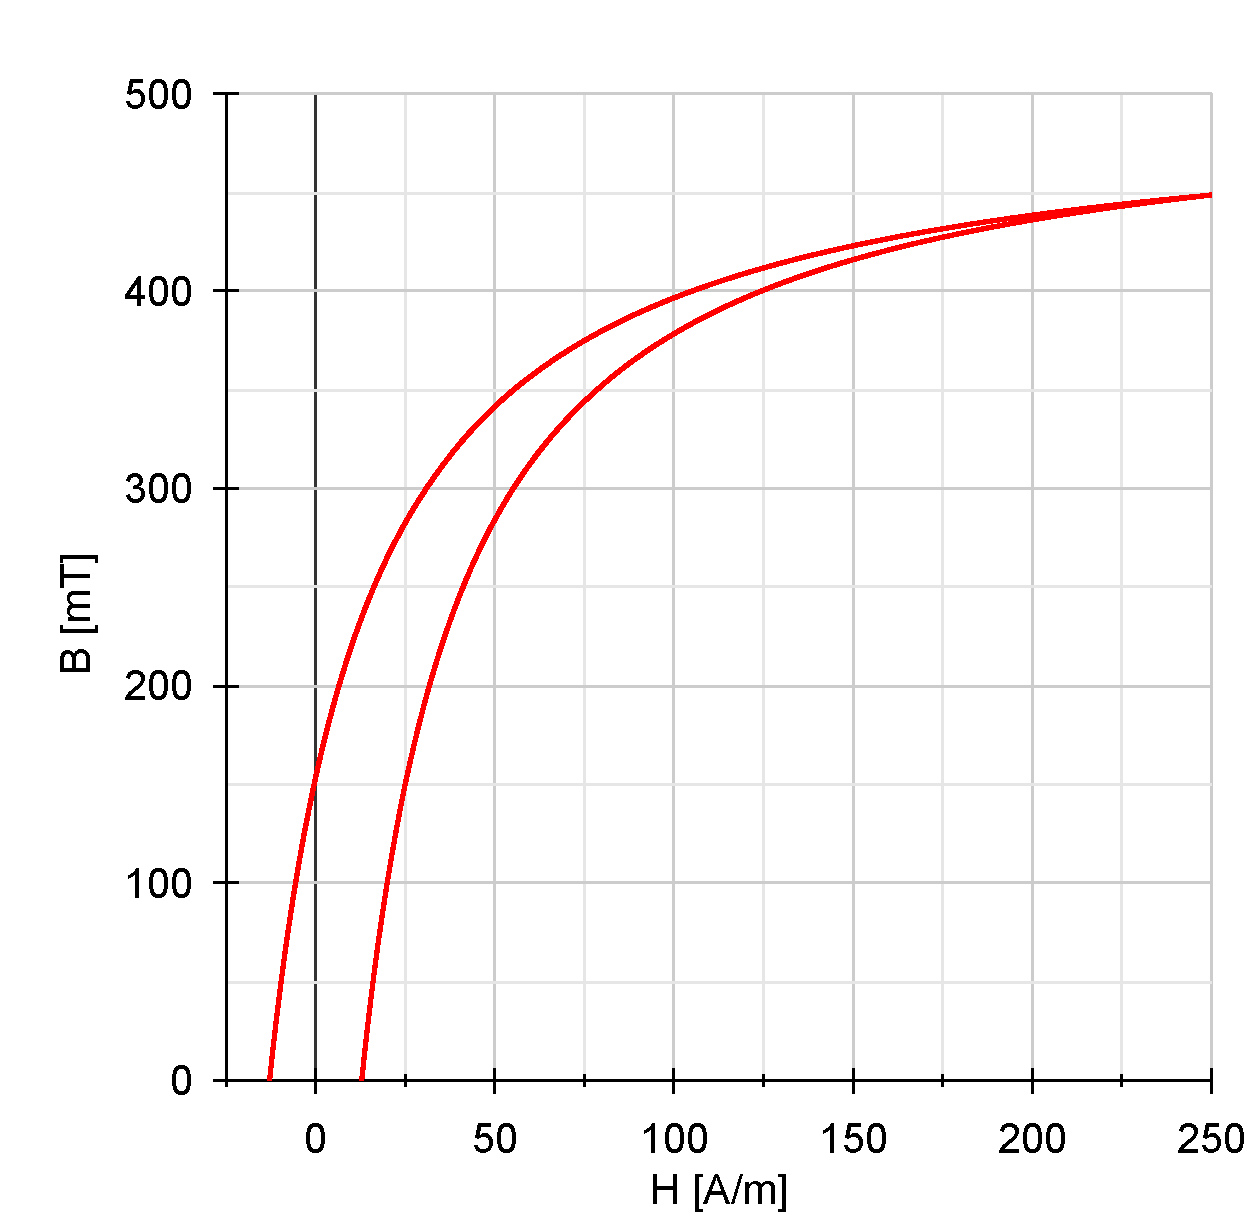
\includegraphics[width=\textwidth]{Bilder/Kapitel3/Hysteresis_LTspice_2.pdf}
        \caption{Simulated hysteresis curve}
    \end{subfigure}
    \begin{subfigure}[b]{0.50\textwidth}
        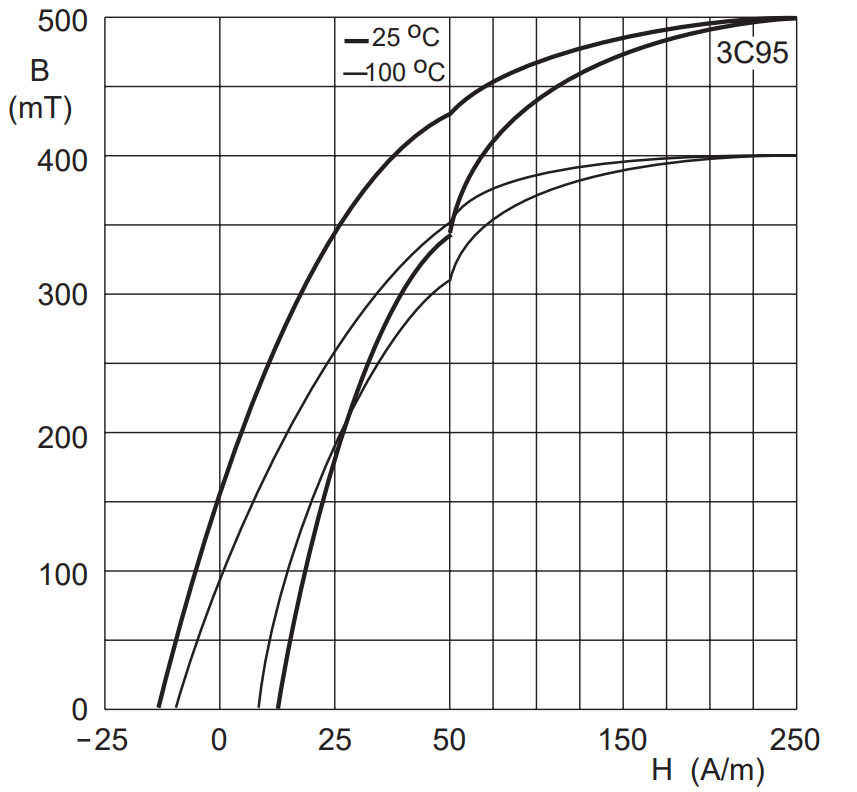
\includegraphics[width=\textwidth]{Bilder/Kapitel3/DataSheet_Hysteresis_Curve.png}
        \caption{Hysteresis given by the datasheet}
    \end{subfigure}
    \caption{Hysteresis comparison}
    \label{fig:hysteresis_comparison}							
\end{figure}
However, since the model is mainly to be used for \ac{DC} offset simulation without the inductor being in saturation, a more telling measurement for the validity of the model is the inductance curve. Using the setup detailed in section \ref{sec:saturation_behaviour_of_the_inductor}, the inductance curve is measured with the Power Choke Tester and simulated in LTspice. Both are plotted in the graph \ref{fig:inductance_measured_and_simulatd}. The inductance values stray far from each other, making this model unsuitable for reliable simulations even when far away from saturation. 
\begin{figure}[H]
    \centering
    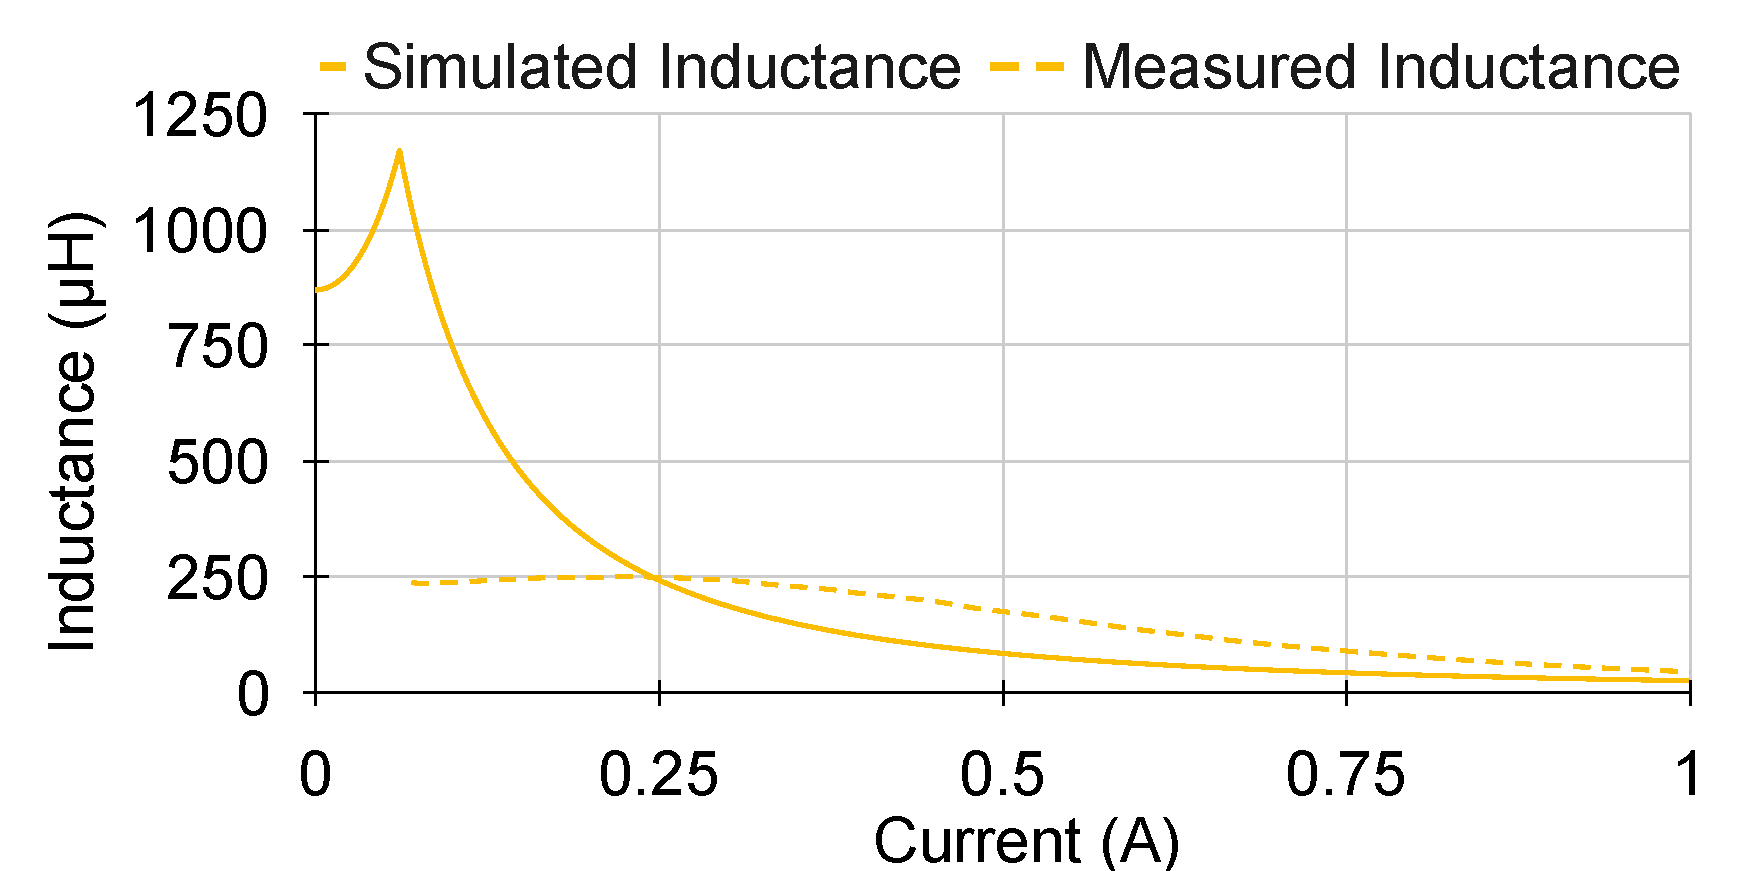
\includegraphics[width=.55\linewidth]{Bilder/Kapitel3/Saturation_Measured_and_Simulated_Hyst.pdf}
    \caption{Inductance measured and simulated}
    \label{fig:inductance_measured_and_simulatd}
\end{figure} 
